\chapter{Satisfiability}
\label{ch:satisfiability}

Satisfiability is the fourth hard-core family and the last technical chapter of
Part~III. It is also the one where the book's machinery is furthest from
sufficient, and saying exactly how far is most of what this chapter does.

The mapping is the easiest in the book: variables are atoms, clauses are
complexes, and a clause forbids exactly one assignment of its members. That is
Chapter~\ref{ch:colouring}'s hypergraph rule with one forbidden configuration
instead of two. But one feature does not carry over, and it decides everything.
Colouring's constraint is symmetric under permuting the colours, so the uniform
message is a fixed point and the threshold has a closed form.
A clause is not symmetric: it forbids a \emph{particular} assignment, the one
its signs pick out. The uniform message is not a fixed point, the disorder has
to be carried, and no closed form survives.

What does survive is a hard-field treatment --- Chapter~\ref{ch:hittingset}'s
warning propagation, on this chygraph --- and it produces one exact result, one
structural statement, and one honest failure. The exact result is the $2$-SAT
threshold. The structural statement is that for $k\ge3$ the trivial fixed point
is stable at \emph{every} clause density, so there is no linear instability at
all. The failure is that the hard field then goes on reporting nothing wrong
well past the point where the formula has stopped being satisfiable.

\section{Clauses as complexes}
\label{sec:clauses}

A $k$-SAT formula over $N$ Boolean variables is a conjunction of $M$ clauses,
each a disjunction of $k$ literals --- a variable or its negation. A clause is
satisfied unless every one of its literals is false, so each clause forbids
exactly one of the $2^{k}$ assignments of its variables. The control parameter
is the clause density $\alpha=M/N$.

The chygraph is immediate. Layer $0$ is the variables, as atoms; layer $1$ is
the clauses, as complexes of cardinality $k$. A variable's chy-degree is the
number of clauses it appears in, so for a random formula it is Poisson with mean
$\ave{\kappa}=k\alpha$: each clause holds $k$ variable slots and there are
$\alpha N$ clauses.

\paragraph{The one thing that is new.} Every complex in this book so far has
carried an interaction that treats its members alike. A clause does not. It
carries $k$ \emph{signs}, and the assignment it forbids depends on them. Two
clauses on the same $k$ variables can forbid different assignments, and in a
random formula they do.

That is quenched disorder living \emph{inside} a complex, and it is the first
time the book has met any. Chapter~\ref{ch:statmech} allowed it without
comment --- Eq.~\eqref{eq:emitted} takes $-\beta H$ as an argument and does not
ask whether it is the same for every complex --- but the consequence is real,
and Sec.~\ref{sec:whatclausetransmits} is it.

\section{What a clause transmits}
\label{sec:whatclausetransmits}

Write $u_{j}$ for the value of variable $j$ that falsifies its literal in clause
$a$. Then the interior sum of Eq.~\eqref{eq:emitted} removes a single
configuration, and
\begin{equation}
  Z_{a\to0}(\sigma_{0})
    =1-\mathbf{1}[\sigma_{0}=u_{0}]\prod_{j\in a\setminus0}\eta_{j}(u_{j}).
  \label{eq:satZ}
\end{equation}
Compare Eq.~\eqref{eq:tauhyp}'s parent, $Z=1-\prod_{j}\eta_{j}(\sigma_{0})$: the
same shape, with the product taken at a fixed assignment rather than along the
diagonal. Satisfiability really is colouring at $q=2$ with the symmetry broken,
and Eq.~\eqref{eq:satZ} is where the breaking enters.

The consequence is worth seeing before any analysis. Put every incoming message
at $\eta=1/2$. Then Eq.~\eqref{eq:satZ} emits $1-2^{1-k}$ on the falsifying
value and $1$ on the other: at $k=3$, $3/4$ against $1$. The emitted message is
\emph{not} uniform, so the uniform message is not a fixed point.

That single fact separates this chapter from the last one. In
Chapter~\ref{ch:colouring} the colour-permutation symmetry gave a uniform fixed
point, Schur's lemma reduced the linearised map to one number, and
Eq.~\eqref{eq:taucol} followed in three lines. Here the symmetry is broken
clause by clause. It is restored only \emph{on average} over the signs, which
means the object that has a symmetric fixed point is the distribution of
messages and not a message. There is no scalar to linearise, and no closed form
of the kind Eq.~\eqref{eq:taucol} provides.

\section{Warning propagation}
\label{sec:sat-wp}

What is available is the hard-field limit, which is Chapter~\ref{ch:hittingset}
transplanted. Keep only whether a message is a \emph{warning}: clause $a$ warns
variable $i$ that $i$ must satisfy $a$, because every other member of $a$ has
already been forced to falsify it.

\begin{calculation}{the warning map, and the factor of one half}
Let $\eta$ be the probability that a clause sends a warning along an inclusion,
and $\pi$ the probability that a variable reached along one is forced to a given
value.

\emph{Down.} A clause warns $i$ only when all $k-1$ other members are forced to
falsify it, so
\[
  \eta=\pi^{\,k-1}.
\]

\emph{Up.} A variable is forced by the warnings arriving from its \emph{other}
clauses. Here the signs enter, and they enter once: a warning arriving at $j$
points at one of the two values, and the chance that it is the value falsifying
the clause under consideration is $1/2$. So with $\bar\Phi$ the excess
chy-degree generating function, the mean number of warnings arriving in the
relevant direction is $\ave{\kbar}\eta/2$, and for Poisson chy-degree
\[
  \pi=\bigl(1-e^{-\ave{\kbar}\eta/2}\bigr)\,e^{-\ave{\kbar}\eta/2},
\]
the two factors being ``at least one warning that way'' and ``none the other
way''. A variable receiving warnings both ways is a contradiction, not a
forcing. Putting the two steps together with $\ave{\kbar}=k\alpha$,
\begin{equation}
  \eta=\Bigl[\bigl(1-e^{-k\alpha\eta/2}\bigr)e^{-k\alpha\eta/2}\Bigr]^{k-1}.
  \label{eq:wp}
\end{equation}
\end{calculation}

Equation~\eqref{eq:wp} is Chapter~\ref{ch:hittingset}'s
Eq.~\eqref{eq:hs} with two changes, and both are worth naming.

The first is the factor $1/2$, and it is the whole of what negatable variables
buy. A hyperedge in Chapter~\ref{ch:hittingset} constrains its members in one
way only; a clause can constrain them either way, so half the warnings a
variable receives are irrelevant to any given clause.

The second is a sign. Chapter~\ref{ch:hittingset}'s map was
order-\emph{reversing}, which is why it needed the $F\circ F$ bracket of
Sec.~\ref{sec:hard} and why plain iteration oscillated. Equation~\eqref{eq:wp}
is order-\emph{preserving}: more warnings force more variables, which send more
warnings. Monotone iteration from zero suffices, exactly as for
Chapter~\ref{ch:cover}'s leaf removal. The two hard-field problems in this book
sit on opposite sides of the sign test that Sec.~\ref{sec:fixedpoint} said would
decide which solver applies, and here is the second of them.

\section{Two-SAT is exact; above it there is no threshold at all}
\label{sec:twosat}

Now linearise Eq.~\eqref{eq:wp} at $\eta=0$. Since $\pi\simeq k\alpha\eta/2$ for
small $\eta$,
\begin{equation}
  \frac{\partial\eta'}{\partial\eta}\bigg|_{0}
    =\lim_{\eta\to0}\Bigl(\frac{k\alpha\eta}{2}\Bigr)^{k-1}\Big/\eta
    =\begin{cases}
       \alpha, & k=2,\\[2pt]
       0, & k\ge3.
     \end{cases}
  \label{eq:satslope}
\end{equation}

\paragraph{$k=2$.} The trivial fixed point loses stability at
\begin{equation}
  \alpha=1,
\end{equation}
and the non-trivial branch grows continuously out of it --- $\eta^{*}=0$ at
$\alpha=0.99$ and $0.0066$ at $\alpha=1.01$. That is the exact $2$-SAT
threshold, which is one of the few thresholds in this subject known rigorously.
It comes out of the general branching condition with no adjustment, and it is
the chapter's benchmark.

\paragraph{$k\ge3$.} The derivative is not small; it is \emph{zero}, at every
clause density. A clause needs $k-1$ warnings at once before it will emit one,
so a single warning cannot start anything, and $\eta\equiv0$ is stable however
many clauses one adds.

This is Sec.~\ref{sec:groupcontagion}'s exclusion, in its purest form. There a
group needed $r\ge2$ infected members and a single seed could not invade; here a
clause needs $k-1$ forced variables and a single warning cannot propagate. The
book has now met the same structure four times --- interdependent networks,
threshold contagion, the Potts model above $q=2$, and satisfiability above
$k=2$ --- and this is the extreme case, because there is no linear instability
anywhere on the axis to mistake for a transition.

The non-trivial branch arrives instead by a fold (Fig.~\ref{fig:sat}). At $k=3$
the map first touches the diagonal at $\alpha=5.39$; below that the only
solution is $\eta=0$.

\begin{figure}[t]
\centering
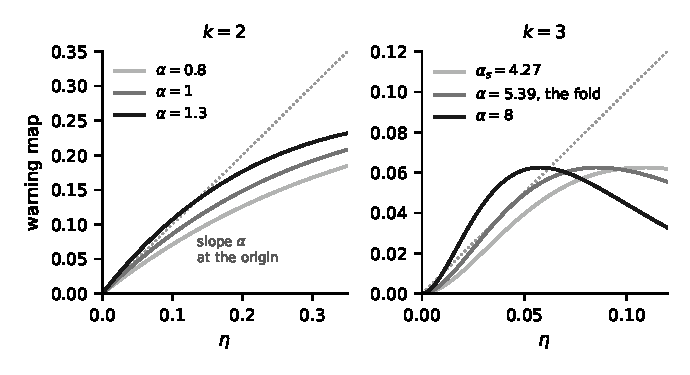
\includegraphics[width=\linewidth]{figs/fig-sat.pdf}
\caption{\textbf{Why two is different.} The warning map,
Eq.~\eqref{eq:wp}, against the diagonal. Left, $k=2$: the map leaves the origin
with slope $\alpha$, so it crosses the diagonal as soon as $\alpha>1$ and the
branch grows continuously. Right, $k=3$: it leaves the origin with slope zero
whatever $\alpha$, so the origin is a fixed point at every density and the
branch can only arrive by a tangency --- here at $\alpha=5.39$, which is well
past the density $\alpha_{s}=4.27$ at which the formula has stopped being
satisfiable. Generated by \code{figs/satisfiability.py}.}
\label{fig:sat}
\end{figure}

\section{Where the hard field is blind}
\label{sec:satblind}

The fold is not the satisfiability threshold, and the gap is the point of this
section.

\begin{center}\small
\begin{tabular}{rrrr}
\hline\hline
$k$ & warning fold & $\alpha_{s}$ & ratio\\
\hline
$2$ & $1.000$ & $1$ & $1.00$\\
$3$ & $5.386$ & $4.267$ & $1.26$\\
$4$ & $18.24$ & $9.931$ & $1.84$\\
$5$ & $61.58$ & $21.12$ & $2.92$\\
\hline\hline
\end{tabular}
\end{center}

The published thresholds are from Ref.~\citep{montanari2008}. Read the last
column: the warning map first notices that something is wrong at a density
$1.26$ times the true one at $k=3$, and nearly three times it at $k=5$. Below
its fold, warning propagation reports no warnings, no contradictions and no
difficulty --- for formulas that are, with probability approaching one,
unsatisfiable.

That is the same defect as Sec.~\ref{sec:hardfail}, one family later and one
degree worse. There, collapsing the field onto an integer discarded an $O(1)$
part and returned a cover of one half where the answer was one third. Here it
discards the same kind of information and the answer is not merely wrong but
uninformative over a wide range of densities.

\paragraph{How much of that number to believe.} Less than the table's digits
suggest, and the chapter had better say which parts are solid.

The two results of Sec.~\ref{sec:twosat} are linearisations, so they do not
depend on how a variable receiving contradictory warnings is counted. The fold
does. Under the strict convention used above --- contradictory warnings are a
contradiction, not a forcing --- the $k=3$ fold is $5.386$; counting instead the
\emph{net} warning field, so that opposing warnings partly cancel, it is
$4.667$. The numbers move by fifteen per cent and more.

What does not move is the direction. Under either convention the fold lies above
$\alpha_{s}$ at every $k$ tried: $4.667$ against $4.267$ at $k=3$, $11.83$
against $9.93$ at $k=4$, $27.91$ against $21.12$ at $k=5$. So the qualitative
statement is robust and the number is a bookkeeping choice, and the table above
should be read as the first and not the second.

\section{Where replica symmetry goes}
\label{sec:sat-rsb}

Random $k$-SAT is the problem for which one-step replica symmetry breaking was
invented, and the reason is visible in the gap just measured.

The correct object is not a single warning probability but a \emph{distribution}
over warnings --- a survey --- and propagating it is survey propagation
\citep{mezard2002science,mezard2002pre}. That calculation returns
$\alpha_{s}=4.267$ for $k=3$, and the intermediate structure that this chapter
cannot see: a clustering transition at $\alpha_{d}=3.86$ where the solutions
shatter into exponentially many groups, and for $k\ge4$ a condensation
transition between the two \citep{montanari2008}.

So the position here is the same as in Chapter~\ref{ch:colouring} but more
acute. There, the replica-symmetric calculation gave a definite closed form that
was a local stability threshold rather than a colourability one. Here even that
is unavailable, because there is no symmetric fixed point to linearise about,
and the hard-field substitute is blind over a range that grows with $k$.

\paragraph{What the chygraph adds, and what it does not.} It adds the structure:
Eq.~\eqref{eq:wp} is written for an arbitrary chy-degree distribution, mixed
clause lengths are one layer per length, and correlations between a variable's
participation in short and long clauses are Sec.~\ref{sec:joint}'s joint
$\Phi$ --- none of which a fixed-$k$, Poisson treatment reaches. It does not add
the one-step calculation, and for this problem that is where the subject
begins rather than ends.

The honest summary is that satisfiability is the model in this book that most
needs what this book does not do. It is included because the mapping is exact
and instructive, because $2$-SAT comes out right, and because the way it fails
is the same way Chapter~\ref{ch:hittingset} failed --- which is worth knowing
about a method one intends to apply elsewhere.

\section{Checks}
\label{sec:sat-checks}

\emph{Against enumeration.} Equation~\eqref{eq:satZ} is checked against a direct
enumeration of a clause's $2^{k}$ assignments for $k=2,3,4$, in rational
arithmetic, including the emitted values at $\eta=1/2$ that establish the
absence of a uniform fixed point.

\emph{Against a rigorous result.} Equation~\eqref{eq:satslope} at $k=2$ gives
$\alpha=1$, the exact $2$-SAT threshold, and the non-trivial branch is confirmed
to be absent at $\alpha=0.99$ and present at $\alpha=1.01$.

\emph{That the derivative really vanishes.} For $k\ge3$ the claim is that a
derivative is zero, which a single finite difference cannot establish. What is
checked is the \emph{rate}: the finite difference at $\varepsilon$ falls like
$\varepsilon^{k-2}$, verified by halving $\varepsilon$ and requiring the ratio
$2^{k-2}$, at $k=3,\dots,6$ and three clause densities each.

\emph{Against the convention.} Both conventions for a contradicted variable are
run. They agree at $k=2$, where the answer is a linearisation, and disagree
above it; both put the fold above $\alpha_{s}$. The chapter quotes the
disagreement rather than one convention's numbers alone.

\emph{What is not checked, because it is not claimed.} Nothing here is a
satisfiability threshold except at $k=2$. Section~\ref{sec:satblind} is the
account of the difference, and Sec.~\ref{sec:sat-rsb} of what would close it.
